\documentclass[a4paper]{book}

%PACKAGES
\usepackage[T1]{fontenc}
\usepackage[utf8]{inputenc}
\usepackage[italian]{babel}
\usepackage{amsfonts} 
\usepackage{amssymb} 
\usepackage{amsmath}
\usepackage{amsthm}		%teoremi
\usepackage{graphicx}	%immagini
\usepackage{setspace}	%interlinea
\onehalfspacing


%THEOREMS, ...
\theoremstyle{definition}
\newtheorem{ex}{Esempio}
\newtheorem{defn}{Definizione}

\theoremstyle{remark}
\newtheorem{oss}{Osservazione}
\newtheorem{dimst}{Dimostrazione}
\newtheorem{idea}{Idea}

\theoremstyle{definition}
\newtheorem{lem}{Lemma}


%NEW COMMANDS
\newcommand{\bbx}{\mathbb{X}}
\newcommand{\bbr}{\mathbb{R}}
\newcommand{\ra}{\Rightarrow}

\title{Calcolo delle variazioni \\ \small{Lezioni di Gobbino 17/18} }
\author{}

\begin{document}

\maketitle
\chapter{Lezione 1}
Il calcolo delle variazioni consiste nello studio di problemi di minimo.
\\
In particolar modo, abbiamo un insieme $\bbx$ ed una funzione $f:\bbx \to \bbr$ e vogliamo trovare min$\{f(x)|x \in \bbx\}$.
\\
Ci sono 4 metodi di approccio al problema:
\\
1.\textbf{Metodo indiretto}	\hspace{3mm}2.\textbf{Metodo diretto} \\
3.\textbf{Rilassamento}	\hspace{3mm}	4.\textbf{Gamma-convergenza}

\begin{ex}
\[
	f:\bbr \to \bbr, f = x^2 - 4x
\]
\[
	\textsf{Metodo indiretto: }f'(x) = 2x - 4 \ra f'(x) = 0 \iff x = 2 \ra \textit{min} = f(2) = -4
\]
Proviamo adesso a dimostrare che $f(x)$ è sempre $\leq$ di $-4$ \footnote{Questa è la vera dimostrazione}.
\[
	x^2 - 4x \ge -4 \iff x^2 -4x + 4 \ge 0 \iff (x -2)^2 \ge 0 
\]
che è vero, inoltre vale l'uguaglianza se e solo se $x = 2$. \\
Metodo diretto: dimostriamo che il minimo esiste, ad esempio usando il teorema di Weierstrass generalizzato:
\[
	f: \bbr \to \bbr \textit{ continua e } \lim_{x \to \pm\infty}f(x) = \infty \ra \textit{il minimo esiste}
\]
Ora che so che esiste posso vedere dove $f'(x) = 0$.
\end{ex}

\begin{ex}
	Cerchiamo min$\{(x^2 - 2)^2 | x \in \mathbb{Q} \}$ \\
	In questo caso il minimo non esiste. Possiamo perciò chiederci: chi è l'inf? Come sono fatte le successioni "minimizzanti"?\\
	L'inf è 0 e le succ. min. hanno una sottosuccessione che tende a $\pm \sqrt 2$.
\end{ex}
\noindent
\textbf{Rilassamento}: Con questo metodo rilassiamo le condizioni imposte dal problema e per farlo possiamo procedere in due modi:
1.Estendo f ad un ambiente più vasto; \\
2.Cambio la funzione in modo che il minimo abbia più probabilità di esistere.	

\begin{ex}
Consideriamo una famiglia di problemi di minimo:
\[
	m_n := min\{e^{x^2} + atg(x) + nsin^2(x)|x \in \bbr^n \}
\]
e chiediamoci:\\
a cosa tende $m_n$ quando $n \to\infty$?\\
a cosa tendono i punti di minimo quando $n \to\infty$?\\
Ci aspettiamo che $m_n \to m_{\infty} := min\{e^{x^2} + atg(x) | x = k\pi, k \in \mathbb{Z} \}$\\
Per rispondere a queste domande usiamo la gamma convergenza.
\end{ex}

\begin{defn}
Generalemente $\bbx$ sarà uno spazio di funzioni. Chiameremo allora 
\[
 	F :\bbx \to \bbr 
 \] 
\textbf{Funzionale}
\end{defn}

\begin{ex}
\[
	F(u) = \int_2^4 (\dot u^2 + sin(u))\,dx
\]
\end{ex}
\noindent
Un particolare tipo di funzionali sono poi quelli $\textbf{integrali}$
\[
	F(u) := \int_a^b L(x, u(x), \dot u(x))\,dx
\]
con $L: [a,b]\times\bbr\times\bbr \to \bbr$.\\
In generale scriveremo $L(x, s, p)$ dette Lagrangiane.\\
Altre generalizzazioni possibili sono:
\[
	F(u) := \int_{a}^{b} L(x, u, \dot u, \ddot u, \dots)dx
\]
\[
	F(u, v) := \int_a^b L(x, u, v, \dot u, \dot v, \dots)dx
\]

\begin{oss}
Problemi più complicati sono del tipo:\\
1.Più variabili in partenza\\
2.Più variabili in partenza e arrivo (caso vettoriale)
\end{oss}

\begin{ex}[Classico]
Data f(x) trovare\\
\[
	min\{\int_a^b \dot u^2 + (u - f)^2\,dx | u \in C^1([a,b])\}
\]

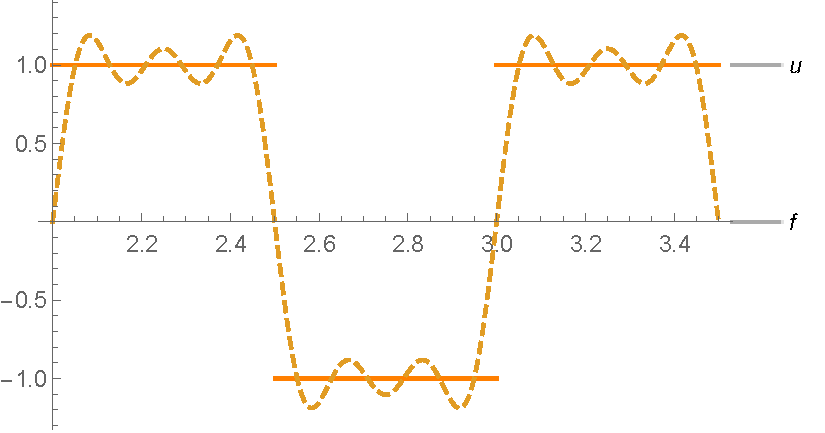
\includegraphics[scale = 0.5]{Fourier_onda_quadra.pdf}\\
\noindent
con f che può essere ad esempio il segnale di un cellulare.
\end{ex}

\begin{ex}[Classico]
\[
	min\{\int_a^b(\dot u^2 + u)dx | u(a) = A, u(b) = B, u \in C^1([a,b])\}
\]
con A e B dati\\
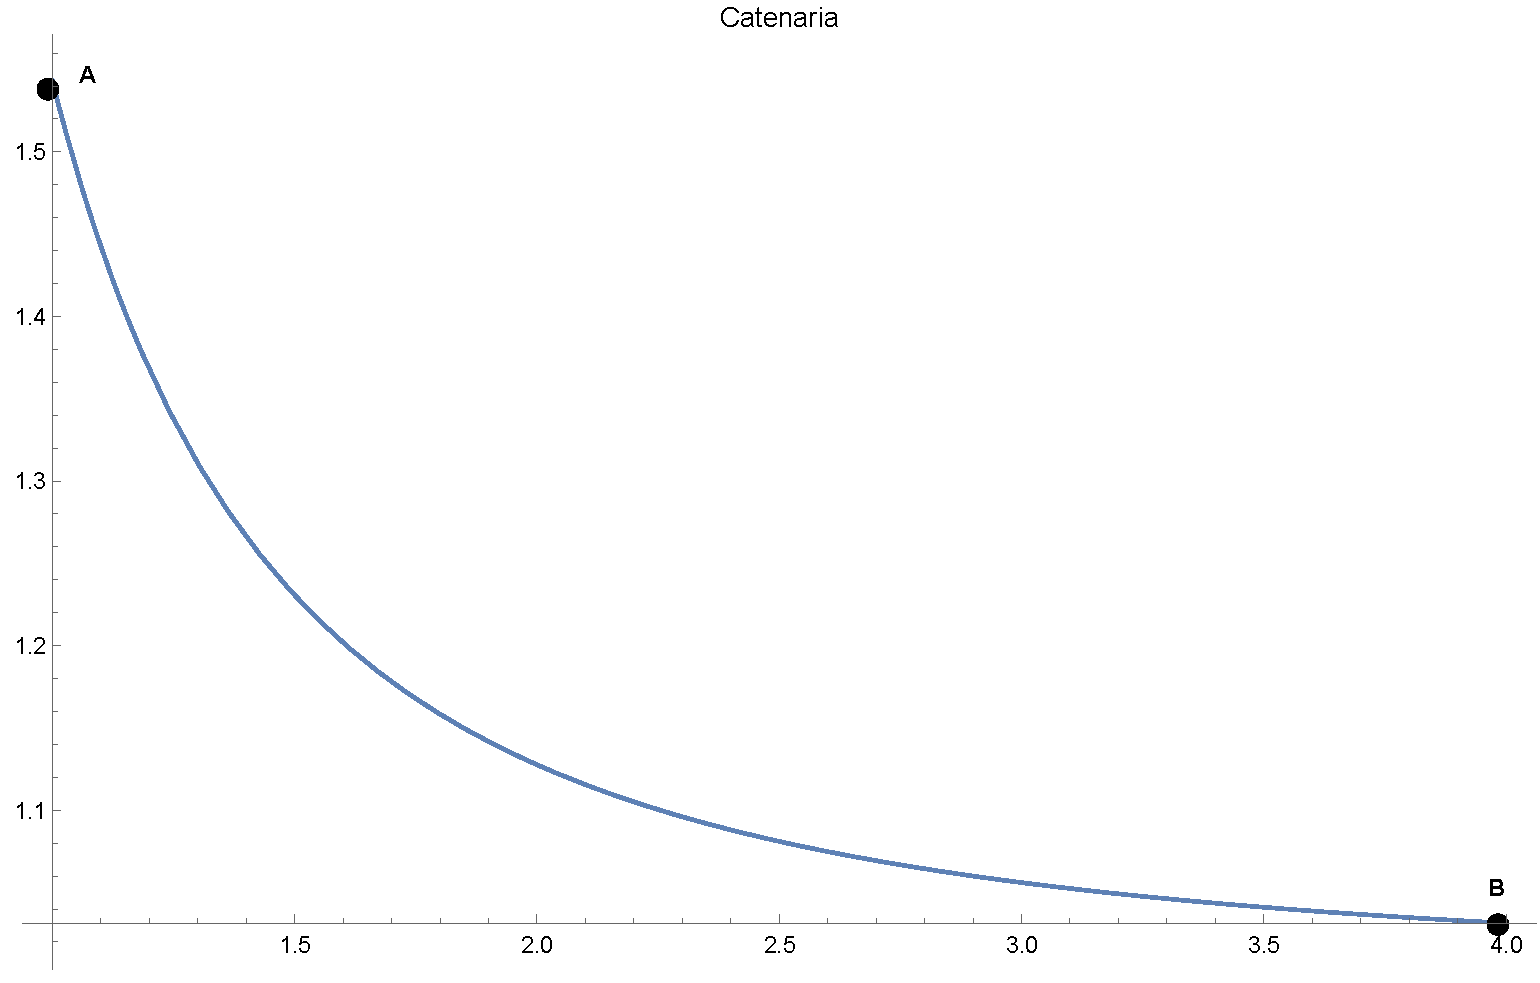
\includegraphics[scale = 0.4]{catenaria.pdf}
\end{ex}

\chapter{Lezione 2}
La variazione prima di un funzionale è l'analogo della derivata prima per una funzione.
\begin{defn}
Consideriamo un insieme $\bbx$ ed $f:\bbx \to \bbr$. Sia $x_0$ un punto di minimo e siano $\delta > 0, \gamma:(-\delta, \delta)\to \bbx$ t.c. $\gamma(0)=x_0$.
Posso considerare la funzione composta
\[
	\varphi(t) := F(\gamma(t)) \in \bbr
\]
Allora
\[
	\varphi:(-\delta, \delta)\to\bbr
\]
con minimo in t=0.\\
Pongo allora $\delta F(x_0, \gamma):=\varphi'(0)$(\footnote{Posto che esista}).\\
$\delta F(x_0, \gamma)$ è detto \textbf{Variazione prima del funzionale F lungo una curva $\gamma$}.
\end{defn}

\begin{oss}
La definizione è valida $\forall x_0$, anche non di minimo, e $\forall$ curva $\gamma : \gamma(0) = x_0$ purchè $\varphi'(0)$ esista.
\end{oss}

\begin{lem}
Se $x_0 \in argmin\footnote{$x \in \bbx$ t.c. f(x) è un minimo} \{f(x)|x\in\bbx \}$, allora 
\[
	\delta F(x_0, \gamma) = 0
\]
quando esiste.
\end{lem}
\noindent 
Supponiamo ora che $\bbx$ sia uno spazio affine con spazio vettoriale di riferimento\footnote{traslato che passa per l'origine, detto anche giacitura} V.\\
In particolare
\[
	\forall u \in \bbx, \forall v \in V \textit{ si ha che } u + v \in \bbx
\]
In questo caso, dati $u_0 \in \bbx$ e $v \in V \smallsetminus \{ 0 \}$ posso considerare la curva
\[
	t \to u_0 + tv : \textit{retta per $u_0$ con direzione v}
\]
e calcolare
\[
	\delta F(u_0, v) := \footnote{"derivata direzionale" o "alla Gateaux"} \lim_{t \to 0} \frac{F(u_0 + tv) - F(u_0)}{t}
\]

\begin{ex}
Consideriamo 3 funzionali
\[
	F(u) = \int_a^b \dot u^2(x)dx \qquad G(u) = \int_a^b |\dot u(x)|dx \qquad H(u) = \int_a^b \sqrt{|\dot u(x)|}dx
\]
con $\bbx = \{u\in C^1([a,b]) | u(a) = A, u(b) = B \}$ 


\begin{oss}
$\bbx$ è uno spazio affine con giacitura
\[
	V = \{v \in C^1([a,b])| v(a) = v(b) = 0\}
\]
\end{oss}
\noindent 
\textit{Metodo indiretto:}
\[
	\varphi(t) = F (u + tv) = \int_a^b(\dot u + t \dot v)^2\,dx = \int_a^b \dot u^2 + \int_a^b 2t\dot u \dot v + \int_a^b t^2 \dot v^2
\]
\[
	\ra \delta F(u, v) := \varphi'(0) \stackrel{\footnote{Deriviamo rispetto a t}}{=}  2\int_a^b \dot u \dot v 
\]
Questa è detta \textbf{Prima forma integrale della variazione prima}.\\
Integriamo adesso per parti:
\[
	\varphi'(0) = 2[\dot u v]_a^b - 2 \int_a^b \ddot u v = \underbrace{2(u(b)v(b)-u(a)v(a))}_{0} - 2\int_a^b \ddot u v = -2\int_a^b \ddot u v
\]
Questa, invece, è detta \textbf{Seconda forma integrale della variazione prima}.

\begin{oss}
Abbiamo usato $\ddot u$ che non è detto esista, ma tanto siamo ancora nella parte preliminare e non devo necessariamente essere formale.
\end{oss}
Allora se $u_0$ è un punto di minimo 
\[
	\int_a^b \dot u_0 \dot v = 0 \qquad \forall v \in V
\]
e se u fosse $C^2$
\[
	\int_a^b \ddot u_0 v = 0 \qquad \forall v \in V
\]
Dalla seconda sembra ragionevole dedurre che 
\[
	\ddot u_0(x) \equiv 0 \ra u_0(x) =\textit{retta } A \to B
\]
Forniamo adesso la dimostrazione rigorosa:\\
Sia $u_0(x)$ la retta e sia $w(x)$ un qualunque altro elemento di $\bbx$. Allora 
\[
	v = w - u_0 \in V
\]
quindi si annulla in a e b.
\[
	F(w) = F(u_0 + v) = \int_a^b (\dot u_0 + \dot v)^2 = \underbrace{\int_a^b \dot u_0^2}_{F(u_0)} + \underbrace{2\int_a^b \dot u_0 \dot v}_{0 \footnote{Integrando per parti poichè $u \in C^2$}} + \underbrace{\int_a^b \dot v ^2}_{\ge 0} \ge F(u_0) \qquad w(x)
\]
Abbiamo così dimostrato che $F(w) \ge F(u_0)$ e vale l'uguale $\iff \int_a^b \dot v^2 = 0\iff\dot v(x) = 0 \iff v(x) = c.te$, ma $v(a)=v(b)=0 \ra v(x)=0 \ra w(x) ) u_0(x)$.\\
Quindi la retta è l'unico punto di minimo 
\[
	\ddot u_0(x) = 0 \qquad \forall x \in [a,b]
\]
Quest'ultima equazione è detta \textbf{Forma differenziale di ELE} \footnote{Equazioni di Eulero-Lagrange}.\\

Passiamo adesso al funzionale H.\\
Dico che $infH = 0$ e non è minimo a meno del caso banale A = B.\\
Infatti
\[
	H(u_n)=\int_{b-1/n}^b |\dot u_n(x)|^2\,dx = \int_{b-1/n}^b |(B-A)n|^{1/2}\,dx = |B-A|^{1/2}\sqrt n \frac1n \to 0 \qquad \textit{per } n \to \infty
\]	
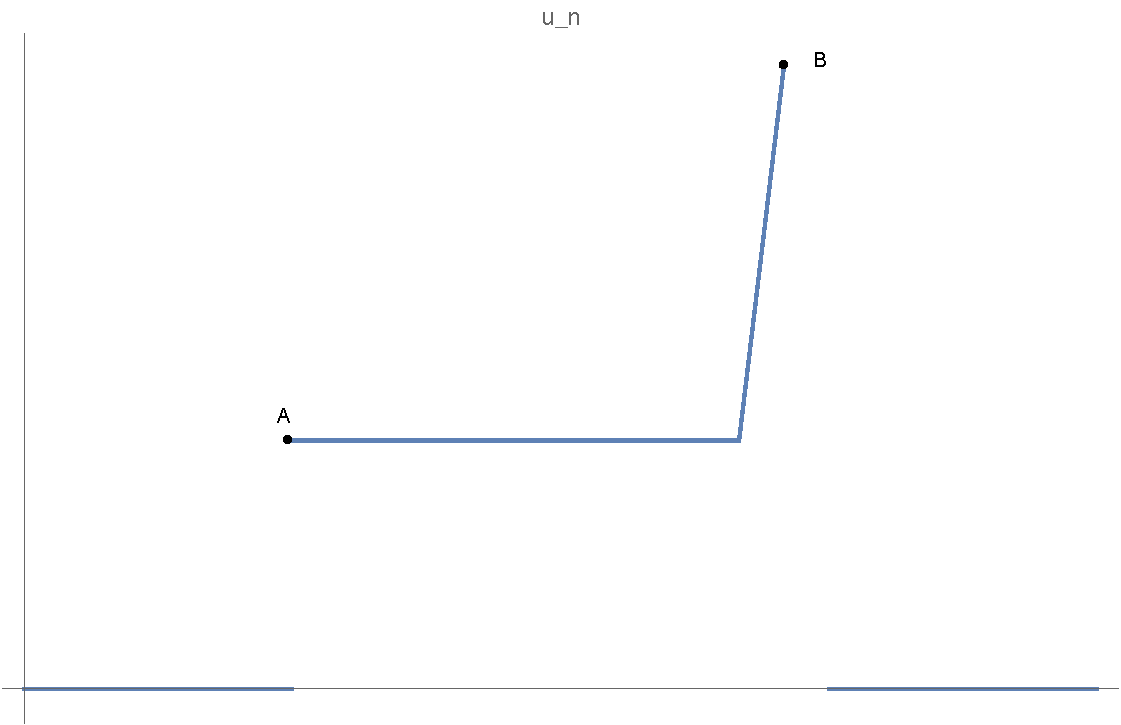
\includegraphics[scale=0.4]{u-n.pdf}

\begin{oss}
Non sarebbe $C^1$, ma fare un piccolo raccordo derivabile conta davvero poco.
\end{oss}

\begin{oss}
Fare l'$inf$ in $C^1, C^{27}, C^\infty$ o $C^1$ a tratti è sempre la stessa cosa, a patto che la Lagrangiana sia continua.
\end{oss}

Con il funzionale $G(u)$ abbiamo che il minimo esiste e i punti di minimo sono tutte le monotone.\\
Supponiamo WLOG B>A. Allora 
\[
	\int_a^b |\dot u(x)|\,dx \ge |\int_a^b \dot u(x)\,dx| = u(b) - u(a) = B-A \qquad \forall u
\]
L'uguaglianza vale se e solo se $\dot u$ ha segno costante.
\end{ex}

\begin{oss}
Lagrangiana:
\begin{itemize}
\item{Strettamente convessa in p $\to$ BUONO}
\item{Non convessa $\to$ GUAI IN VISTA}
\item{Convessa, ma non strettamente $\to$ RISCHI UNICITA' E REGOLARITA'}
\end{itemize}
\end{oss}

\chapter{Lezione 3}
\begin{lem}[Fondamentale del calcolo delle variazioni (FLCV)]
Sia $f: [a,b] \to \bbr$ continua.\\
Supponiamo che 
\[
	\int_a^b f(x)v(x)\,dx = 0 \qquad \forall v \in C^\infty_c ([a,b])	
\]
Allora 
\[
	f(x) \equiv 0 \quad \textit{in } [a,b]
\]
\end{lem}

\begin{defn}[Funzioni a supporto compatto]
$C^\infty_c ([a,b])$ implica che $\exists [c,d] \subset (a,b)$ t.c. $v(x) = 0$ fuori da $[c,d]$ (supporto compatto)
\end{defn}
Vediamo due dimostrazioni per questo teorema
\begin{dimst}[Per assurdo]
Supponiamo f non identicamente nulla, allora WLOG $\exists x_0 \in (a,b)$ t.c. $f(x_0) > 0~$(altrimenti prendo -f).\\
Allora per continuità $\exists \delta > 0$ t.c. $f(x) \ge \frac12 f(x_0) \forall x \in B(x_0, \delta$.\\
Prendo ora $v \in C^\infty (\bbr)$ t.c. 
\[
v(x) = \footnote{La $C^\infty$-tizzo} 
\begin{cases}
v(x) = 1 & x \in B(x_0, \delta) \\
v(x) = 0 & \text{altrove}
\end{cases}
\]
Allora 
\[
	\int_a^b f(x)v(x)\,dx = \int_{x_0 - \delta}^{x_0 + \delta} f(x)v(x)\,dx > 0
\]
ASSURDO \qed
\end{dimst}

\begin{dimst}[Per approssimazione]
\begin{idea}
Se
\[ 
\int_a^b f(x)v(x) = 0 \quad \forall v \in C^\infty_c \ra \int_a^b f(x)v(x)=0 \quad v\in C^0
\]
\end{idea}	
Supponendo vero questo, prendiamo 
\[
	v(x) \equiv f(x) \ra \int_a^b f^2(x) = 0 \iff\footnote{Integriamo una funzione sempre positiva} f(x)=0
\]
Fatto di approssimazione: $\forall v:[a,b] \to \bbr$ continua, esiste una successione di funzioni $\{v_n\} \subseteq C^\infty_c((a,b))$ t.c.\\
1. $\exists M$ t.c. $|v_n(x)| \le M \quad \forall n \in \mathbb{N} \quad\forall x \in [a,b] $ (poichè v continua)\\
2. $v_n(x) \stackrel{u}{\to} v(x)$ sui compatti $K \subset (a,b)$\\
Questo basta per concludere che 
\[
	\lim_{n \to \infty}\int_a^b v_n(x)f(x)\,dx = \int_a^b v(x)f(x)\,dx
\]
\textit{Fisso $\epsilon > 0$ e ho convergenza degli integrali in $[a+\epsilon, b- \epsilon]$. Gli integrali in $[a, a+\epsilon],[b- \epsilon, b]$ si stimano per equilimitatezza.}
\end{dimst}

\begin{oss}[Generalizzazioni]
Possiamo adesso chiederci per quali classi di funzioni V vale il lemma?\\
1. Se l'integrale è nullo $\forall v \in V$, allora è nullo $\forall v \in Span\{v\}$.\\
2. Se l'integrale è nullo $\forall v \in V$, allora è nullo sulla chiusura di V rispetto alla convergenza uniforme sui compatti contenuti in $[a,b] \smallsetminus \{\text{numero finito di punti}\} $. (si dimostra per approssimazione).
\end{oss}

Il lemma allora funziona per tutti gli spazi t.c. $\overline{Span\{v\}} = C^0 $.

\begin{lem}[Du Bois-Reymond (DBR)]
Sia $f:[a,b]\to\bbr $ continua. Supponiamo che 
\[
	\int_a^b f(x)v(x)\,dx = 0\quad \forall v \in C^\infty_c((a, b)) \text{ t.c. } \int_a^b v(x)\,dx = 0
\]
Allora
\[
	f(x) \equiv \text{ c.te } \quad \text{ in } [a,b]
\]
\end{lem}

\begin{dimst}[Per assurdo]
\begin{idea}
Se f soddisfa l'ipotesi allora anche $f(x) + c$ la verifica $\forall c \in \bbr$
\end{idea}
Sia f non costante, allora WLOG $\exists x_0,y_0 $ t.c. $f(x_0) < f(y_0)$.\\
A meno di aggiungere una costante, posso assumere $f(x_0) = -f(y_0)$.\\
Considero allora v del tipo\\ 
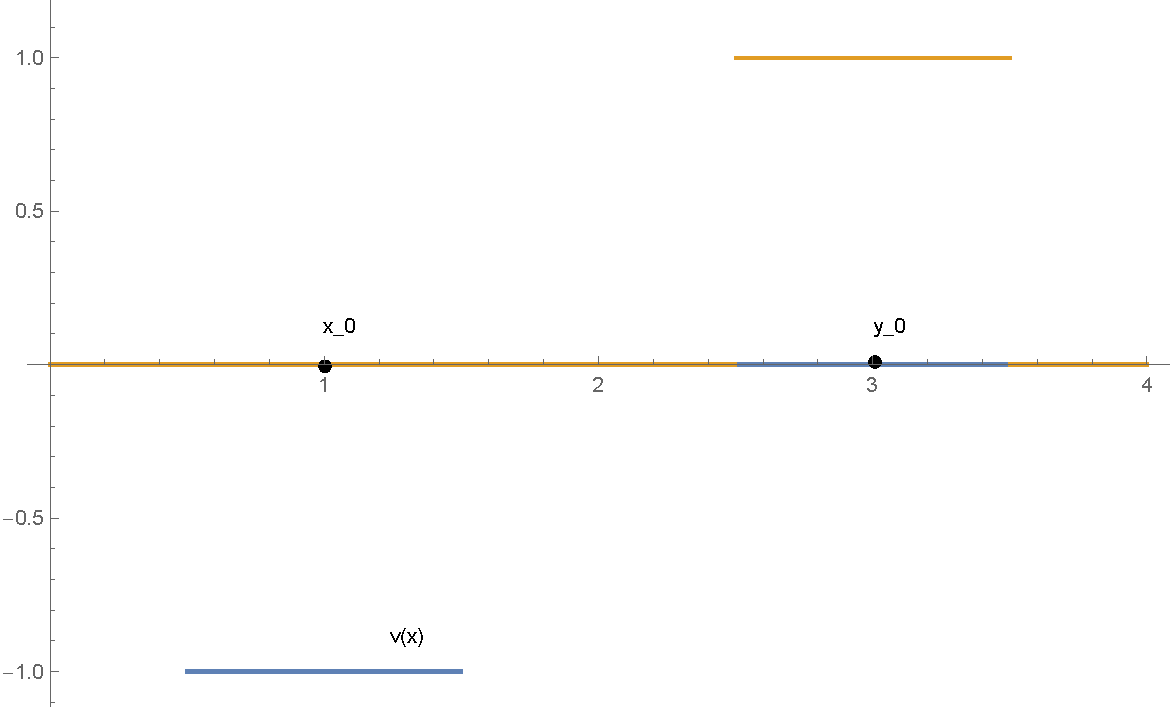
\includegraphics[scale=0.4]{dbr.pdf}
dove v è simmetrica.\\
Allora
\[
	\int_a^b f(x)v(x)\,dx > 0
\]
ASSURDO \qed
\end{dimst}

\begin{dimst}[Per approssimazione]
Si dimostra che ogni funzione $v \in C^0$ a media nulla si può approssimare con funzioni $v \in C^\infty_c((a,b))$ a media nulla e quindi 
\[
	\int_a^b f(x)v(x)\,dx = 0\quad \forall v \in C^\infty_c \text{ con } \int_a^b v(x) = 0 
\]
\[
	\ra \int_a^b f(x)v(x)\,dx = 0 \quad \forall v \in C^0 \text{ con } \int_a^b v(x)\,dx = 0
\]
A questo punto prendo $c \in \bbr $ t.c. $\int_a^b (f(x)+c)\,dx = 0$ e uso $v(x) = f(x)+c$. Ottengo quindi che $f(x) + c \equiv 0 \ra f(x)$ è costante. \qed
\end{dimst}
Anche in questo caso posso usare classi più ristrette di funzioni.\\
\begin{ex}
\[
	min\{\int_0^2 \dot u^2\,dx |\underbrace{ u(0) = 0, u(2) = 5, \int_0^2 u(x)\,dx = 7}_{\bbx}\}
\]
Osserviamo che $\bbx$ è uno spazio affine con giacitura
\[
	V := \{v \in C^1([0,2])|v(0) = 0, v(2) = 0, \int_0^2v(x)\, dx = 0 \}
\]
Data $u \in \bbx$ e $v \in V$ calcolo
\[
	F(u + tv) = F(u) + 2t \int_0^2 \dot u \dot v + t^2\int_0^2\dot v^2
	\ra \delta F(u,v) = \lim_{t\to0} \frac{F(u+tv)-F(u)}t = 2\int_0^2\dot u \dot v
\]
Integrando per parti e supponendo $u \in C^2$ troviamo
\[
	\delta F (u,v) = -2 \int_0^2 \ddot u v
\]
Quindi se u è un punto di minimo deve verificare
\[
	\int_0^2 \ddot u v = 0
\]
\[
	\forall v \in C^1([0,2]) \text{ t.c. } \int_0^2v(x) = 0, v(0)=v(2)=0
\]
Possiamo allora applicare il lemma DBR e quindi $\ddot u = $ costante $\ra u(x) = ax^2+bx+c$.\\
Imponendo le 3 condizioni trovo poi a,b,c.\\
Una volta trovato il punto di minimo faccio la dimostrazione con la disuguaglianza.
\end{ex}
\begin{lem}[DBR altro enunciato]
\[
	\int_a^b f(x)\dot v(x)\, dx = 0\quad \forall v \in C^\infty_c((a,b))
\]
Allora
\[
	f(x) \equiv \text{ c.te in } [a,b]
\]
\end{lem}

\begin{dimst}
Basta osservare che le funzioni $\dot v$ con $v \in C^\infty_c((a,b))$ sono tutte e sole le $w \in C^\infty_c$ a media nulla (l'integrale è ka differenza tra i valori agli estremi).
\end{dimst}

\begin{ex}
\begin{enumerate}
\item{$\int_a^b fv = 0\quad \forall v \in C^\infty_c \text{ t.c. } \int_a^b v = 2017 $}
\item{$\int_a^b f \ddot v = 0\quad v \in C^\infty_c $}
\end{enumerate}
\begin{enumerate}
\item{$f = 0$, la dimostrazione è analoga a quella per v a media nulla}
\item{$f(x)$ è una funzione affine del tipo $ax + b$}
\end{enumerate}
\end{ex}
\end{document} 